\documentclass[a4paper,11pt]{scrartcl}
\usepackage[T1]{fontenc}
\usepackage[utf8x]{inputenc}
\usepackage{graphicx}
\usepackage{xcolor}

% \usepackage{tgheros}
% \usepackage[defaultmono]{droidmono}

\usepackage{amsmath,amssymb,amsthm,textcomp}
\usepackage{enumerate}
\usepackage{multicol}
\usepackage{tikz}

\usepackage{menukeys}

\usepackage{geometry}
\geometry{total={210mm,297mm},
left=25mm,right=25mm,%
bindingoffset=0mm, top=20mm,bottom=30mm}

\linespread{1.2}

\newcommand{\linia}{\rule{\linewidth}{0.5pt}}

% my own titles
\makeatletter
\renewcommand{\maketitle}{
\begin{center}
\vspace{2ex}
{\huge \@title}
\vspace{1ex}
\\
\linia\\
\@author \hfill \@date
\vspace{4ex}
\end{center}
}
\makeatother
%%%

% custom footers and headers
\usepackage{fancyhdr}
\pagestyle{fancy}
\lhead{}
\chead{}
\rhead{}
\lfoot{\mytitle}
\cfoot{}
\rfoot{\thepage}
\renewcommand{\headrulewidth}{0pt}
\renewcommand{\footrulewidth}{0.5pt}

%

% code listing settings
\usepackage{listings}
\lstset{
    language=Python,
    basicstyle=\ttfamily\small,
    aboveskip={1.0\baselineskip},
    belowskip={1.0\baselineskip},
    columns=fixed,
    extendedchars=true,
    breaklines=true,
    tabsize=4,
    prebreak=\raisebox{0ex}[0ex][0ex]{\ensuremath{\hookleftarrow}},
    frame=lines,
    showtabs=false,
    showspaces=false,
    showstringspaces=false,
    keywordstyle=\color[rgb]{0.627,0.126,0.941},
    commentstyle=\color[rgb]{0.133,0.545,0.133},
    stringstyle=\color[rgb]{01,0,0},
    numbers=left,
    numberstyle=\small,
    stepnumber=1,
    numbersep=10pt,
    captionpos=t,
    escapeinside={\%*}{*)}
}

% Inline graphics
\usepackage{graphicx,calc}
\newlength\myheight
\newlength\mydepth
\settototalheight\myheight{Xygp}
\settodepth\mydepth{Xygp}
\setlength\fboxsep{0pt}
\newcommand*\inlinegraphics[1]{%
  \settototalheight\myheight{Xygp}%
  \settodepth\mydepth{Xygp}%
  \raisebox{-\mydepth}{\includegraphics[height=\myheight]{#1}}%
}

% Swift
\lstdefinelanguage{swift}
{
  morekeywords={
    func,if,then,else,for,in,while,do,switch,case,default,where,break,continue,fallthrough,return,
    typealias,struct,class,enum,protocol,var,func,let,get,set,willSet,didSet,inout,init,deinit,extension,
    subscript,prefix,operator,infix,postfix,precedence,associativity,left,right,none,convenience,dynamic,
    final,lazy,mutating,nonmutating,optional,override,required,static,unowned,safe,weak,internal,
    private,public,is,as,self,unsafe,dynamicType,true,false,nil,Type,Protocol,
  },
  morecomment=[l]{//}, % l is for line comment
  morecomment=[s]{/*}{*/}, % s is for start and end delimiter
  morestring=[b]" % defines that strings are enclosed in double quotes
}
\definecolor{keyword}{HTML}{BA2CA3}
\definecolor{string}{HTML}{D12F1B}
\definecolor{comment}{HTML}{008400}
\lstset{
  language=swift,
  basicstyle=\ttfamily,
  showstringspaces=false, % lets spaces in strings appear as real spaces
  columns=fixed,
  keepspaces=true,
  keywordstyle=\color{keyword},
  stringstyle=\color{string},
  commentstyle=\color{comment},
}
\lstset{language=Swift}

\begin{document}

\newcommand{\mytitle}{TP 4 - Clock}
\title{\mytitle}
\author{Adrien Humilière}
\date{29/03/2018}

\maketitle

\section*{Part 1}

\begin{itemize}
\item In Interface Builder, add a text label for displaying the current time onto the view.
\item Apply styles, adjust position, add autolayout constraints, and set the initial text value to \textbf{00:00}.
\item Some methods of the view controllers are automatically called by the application, following it's lifecycle events, such as \texttt{viewDidLoad}. Experiment with generating an explicit console message with \texttt{print()} during \texttt{viewDidLoad}.
\item Run the app, and witness the print message on the console.
\item Experiment changing the label text during \texttt{viewDidLoad}.
\end{itemize}

\section*{Part 2}

\begin{itemize}
\item Most of iOS applications follow the MVC pattern. Model, views and controllers have separated roles :
\begin{description}
\item[Model] Manages data and only data.
\item[View] Manages the display of informations to the user.
\item[Controller] Picks data from the model, format it and send it to the view for display.
\end{description}
\item In that case, we need a model to encapsulate the representation of a clock. Add a \texttt{Clock} class to the project.
\item Using the Xcode Documentation and API Reference, explore the \texttt{Date} class.
\item Define and implement a \texttt{currentTime} method that will return a \texttt{Date} object of the current time. This method should always return a new instance of \texttt{Date}.
\item For case like this \texttt{currentTime} method, Swift provides a feature known as "computed properties" that represent properties whose values are computed each time they are accessed. Replace the currentTime method definition with a computed property.
\begin{lstlisting}
var currentTime: Date {
	return ...
}
\end{lstlisting}
\item Declare a \texttt{clock} property within the \texttt{ViewController} class, with an instance of \texttt{Clock} as default value.
\item Update \texttt{viewDidLoad} to set the label text with the raw \texttt{Date} object returned by the \texttt{Clock} \texttt{currentTime} property.
\item Run the app. You may witness that we need to customize the format of the \texttt{Date} as a string.
\item Using the Xcode Documentation and API Reference, explore the \texttt{DateFormatter} class and the \texttt{DateFormatterStyle} constants. Use a \texttt{DateFormatter} to display a properly formatted time on the screen.
\begin{lstlisting}
let formatter = DateFormatter()
formatter.timeStyle = .short
timeLabel.text = formatter.string(from: clock.currentTime)
\end{lstlisting}
\item Run the app, and witness the correctly formatted time on the screen. Experiment changing the simulator locale in various languages/regions (in iOS settings) and run the application again.
\end{itemize}

\section*{Part 3}

\begin{itemize}
\item Using the Simulator, send the app to the background (\keys{\shift+\cmd+h}), wait until the OS X menu bar time indicator has changed, and bring the app to the foreground. Observe that the time is not current.
\item Using the Multitasking Bar (\keys{\shift+\cmd+h}, twice quickly), force quit the app and start it again. Notice the time is now correct. The time is correct only when starting the application.
\item Add a \texttt{print()} call in \texttt{viewDidLoad}.
\item Run the app, and observe the Xcode console while repeating the starting, backgrounding, foregrounding and quitting of the app. When does the iOS app seems to execute this \texttt{viewDidLoad} method?
\item Examine the class declaration for \texttt{ViewController} and not that it extends \texttt{UIViewController}.
\item Using the Xcode Documentation and API Reference, explore the \texttt{UIViewController} class reference and notice its life cycle methods.
\item Experiment with attempting to set the current time by overriding \texttt{viewWillAppear:}.
\item Run the application. Observe the Xcode console while foregrounding and backgrounding the app. Notice how \texttt{viewWillAppear:} is also not the appropriate lifecycle method.
\item Using the Project Navigator, examine \texttt{AppDelegate.swift}. The app delegate implements the UIApplicationDelegate protocol and will receive all events corresponding to the application lifecycle. Check this methods in the documentation.
\item Instead of adding a print call to all \texttt{AppDelegate} methods, use Xcode to add breakpoints that automatically continue after writing a message to the console.
\begin{figure}[h]
	\begin{center}
   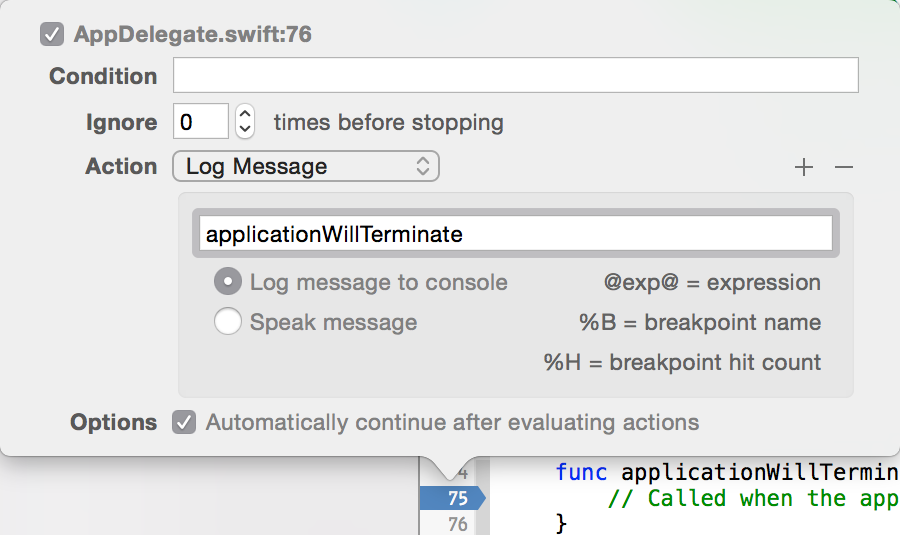
\includegraphics[width=200pt]{breakpoint.png}
	\end{center}
\end{figure}
\item Observe the Xcode console while starting, backgrounding, foregrounding, quitting and restarting the app.
\item Choose the event that suite best for the feature of updating the currently displayed time. However, the controller should be responsible for communicating with the view, and writing view-related code in the \texttt{AppDelegate} violate the separation of concerns of the MVC pattern.
\end{itemize}

\section*{Part 4}

\begin{itemize}
\item The \texttt{NotificationCenter} allow us to observe system and application events, from anywhere in the application (this is not the same as user notifications).
\item Explore the \texttt{NotificationCenter} class documentation, its \texttt{default} class method and the \texttt{addObserver:selector:name:object:} method.
\item Register the controller as an observer in \texttt{viewDidLoad}. This registration will make the system call a \texttt{updateTimeLabel} when the application will enter foreground.
\begin{lstlisting}
NotificationCenter.default.addObserver(self, 
	selector: Selector("updateTimeLabel"), 
	name: NSNotification.Name.UIApplicationWillEnterForeground, 
	object: nil)
\end{lstlisting}
\item Implement the \texttt{updateTimeLabel} method.
\item Refactor \texttt{viewWillAppear} to use \texttt{updateTimeLabel}.
\item Run the app and use the Simulator to send the app to the background (\keys{\shift+\cmd+h}). Wait until the OS X menu bar time indicator has changed, and bring the app to the foreground. Observe that the time is current.
\item Experiment with using an invalid selector name when registering an observer in viewDidLoad. Run the app, send the app to the background, bring the app to the foreground, and observe the app crashing. Restore the correct selector name.
\item It is a best practice to unregister observers when an application quits or is "destroyed" from memory Unregister the observer in a deinitializer.
\begin{lstlisting}
deinit {
	NSNotificationCenter.default.removeObserver(self)
}
\end{lstlisting}
\item The app delegate has no controller-related responsibilities, and the view controller encapsulates the coordination of updating the view.
\end{itemize}

\section*{Part 5}

\begin{itemize}
\item Imagine a real user of the Clock application. What is the main flaw of the app? time is only updated when bringing the app into the foreground, and the displayed time does not continuously change while the app is running.
\item Add a new controller property for an optional \texttt{Timer}. The \texttt{timer} property is declared as an optional, because the \texttt{ViewController} initializer will not initialize the property.
\item Explore the \texttt{Timer} class documentation and its \\\texttt{scheduledTimerWithTimeInterval:target:selector:userInfo:repeats:} class method.
\item Replace the observer registration in \texttt{viewDidLoad} with the creation of a \texttt{Timer} that will call \texttt{updateTimeLabel} every second.
\begin{lstlisting}
Timer.scheduledTimer(timeInterval: 1.0, 
	target: self, 
	selector: Selector("updateTimeLabel"), 
	userInfo: nil, 
	repeats: true)
\end{lstlisting}
\item Modify the \texttt{updateTimeLabel} method's format of the displayed time (\texttt{formatter.timeStyle}), such that it displays seconds. Choose the relevant time style.
\item Replace the observer removal in the deinitializer with an invalidation of the timer.
\begin{lstlisting}
deinit {
	if let timer = self.timer {
		timer.invalidate()
	}
}
\end{lstlisting}
\item Run the app and observe that it continuously displays the current time.
\end{itemize}

\section*{Part 6}

\begin{itemize}
\item The iOS Human Interface Guidelines, or "HIG", describes best practices for consistent, high quality user experience. Explore this documentation : https://developer.apple.com/ios/human-interface-guidelines. It should be followed for your project.
\item It is best practice to not hiding the iOS status bar, but we should make the design decision to hide the status bar for this app in order to remove the redundancy of the status bar's time display.
\item An individual view controller can override a \texttt{prefersStatusBarHidden} method, and the status bar can be disabled application-wide through configuration.
\item Using the Project Navigator, select \texttt{Info.plist}, add a new \texttt{Boolean} item called \texttt{Status bar is initially hidden} and assign it the value \texttt{YES}. Add a second \texttt{Boolean} item called \texttt{View controller-based status bar appearance} and assign it the value NO.
\item Run the app, and observe how the status bar is now hidden.
\end{itemize}


\end{document}
